En Amérique centrale, les Mayas utilisaient un système de numération comprenant trois signes.

\begin{center}
	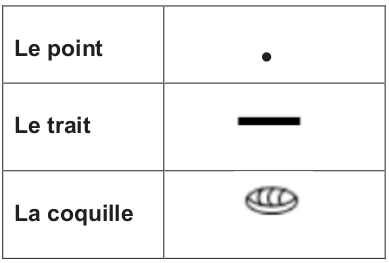
\includegraphics[width=.4\textwidth]{./images/2022-g2-ex5-img1.png}
\end{center}

\textbf{Le signe « coquille » indique l’absence de quantité.}

Quelques correspondances entre écriture Maya et écriture décimale sont données dans le
tableau ci-dessous :

\begin{center}
	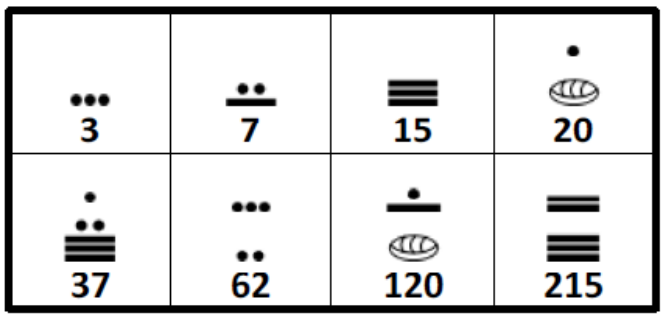
\includegraphics[width=.6\textwidth]{./images/2022-g2-ex5-img2.png}
\end{center}

\begin{enumerate}
\item Donner la valeur du signe « point » et celle du signe « trait » dans l’écriture de $7$ ?
\item Le système maya est un système vigésimal (système qui a pour base $20$). Donner
l’écriture maya du nombre $21$.
\item Justifier l'écriture maya du nombre $37$.
\item Donner l'écriture des deux nombres suivants dans notre système de numération.\par 
\begin{minipage}{3cm}
\begin{enumerate}
	\item 
\includegraphics[width=.7\textwidth]{./images/2022-g2-ex5-img3.png}
\end{enumerate}
\end{minipage}
\begin{minipage}{3cm}
\begin{enumerate}
	\setcounter{enumii}{1}
	\item 
\includegraphics[width=.6\textwidth]{./images/2022-g2-ex5-img4.png}
\end{enumerate}
\end{minipage}
\item 
\begin{enumerate}
	\item Donner l'écriture maya du nombre $25$.
	\item Donner l'écriture maya du nombre $101$.
	\item Le système de numération maya est qualifié, tout comme le système de numération
que nous utilisons, de système positionnel. Expliquer pourquoi.
\end{enumerate}
\end{enumerate}